\documentclass[10pt]{exam}
\usepackage[phy]{template-for-exam}
\usepackage{tikz,tikzpingus,graphicx}
\pinguloadlibrary{horse}
\usetikzlibrary{shadings,decorations.pathmorphing,arrows.meta,patterns}

\def\headsize{0.4}
      \def\elevatorwidth{2.5}
  
      \tikzstyle{person}=[ultra thick, orange!50, scale=0.8]
  
      \tikzset{
        elevator/.pic = {
          \begin{scope}[scale=0.8]
            \draw[fill=gray!30] 
              (-.2,-.05) rectangle (\elevatorwidth+.2,3.55);
            \draw[fill=white] 
              (0,0) rectangle (\elevatorwidth,3.5);
    
            %guide-line (for development)
            %\draw (\elevatorwidth/2,0) -- ++(0,4);
    
    
            \path (\elevatorwidth/2,3.9) coordinate (pulley);
            \draw (pulley) -- ++(0,-0.4);
            \filldraw[fill=gray] (pulley) circle (0.3);
            \filldraw[fill=gray!50] (pulley) circle (0.2);
            \draw[thick] (pulley) 
              ++(-0.3,1) --
              ++(0,-1)
              arc[start angle=-180, end angle=0, radius=0.3] --
              ++(0,1);
          \end{scope}
        }
      }

\title{Weight Questions}
\author{Rohrbach}
\date{\today}

\begin{document}
\maketitle

\begin{questions}

\question
  Consider a 12-kg bowling ball.
  \begin{parts}
    \part
      What is the bowling ball's weight on earth? \vs

    \part
      What is the bowling ball's weight on Mars where $g=\SI{3.71}{\meter\per\second^2}$? \vs
  \end{parts}

  
\question
  In the famous Leaning Tower of Pisa experiment, Galileo dropped two balls from the top of the tower.  Let's say that one was 5~kg and the other was 500~kg

  \begin{parts}
    \part Calculate the weight of the 5-kg ball. \vs
    \part Calculate the weight of the 500-kg ball. \vs
    \part Newton's Second Law says that the ball with more force (\emph{i.e.} more weight) should have a greater acceleration.  How can both balls have the same acceleration?
  \end{parts}

  \begin{tikzpicture}
    \node[anchor=north east] at (0,0) {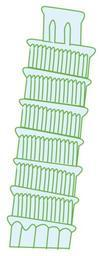
\includegraphics[scale=0.3]{pisa.jpg}};
    \draw[fill=gray] (0.2,-0.5) circle (0.1);
    \draw[fill=gray] (1,-0.5) circle (0.3);

  \end{tikzpicture}

  \vs


\pagebreak

\question
When you are riding in an elevator, there are some times that you feel heavier and some times that you feel lighter.


  \begin{parts}

    \part Let's say your mass is 95~kg.  Calculate the weight (that is, force of gravity) acting on you. \vs

    \part When you stand in a stationary elevator, are you in mechanical equilibrium?  Draw the Free-Body diagram.


      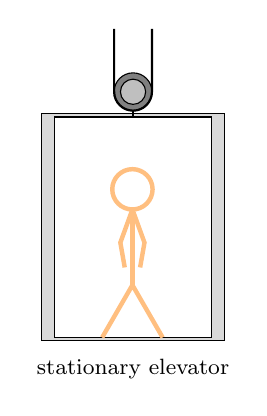
\begin{tikzpicture}[scale=0.8]

          \path (0,0) pic{elevator} coordinate (start);

          \begin{scope}[person]
            \draw (start) 
            ++(.95,0) coordinate (left foot) --
            ++(60:1.2) coordinate (waist) --
            ++(-60:1.2) coordinate (right foot);

            \draw (waist)
              -- ++(90:1.5) coordinate (neck);
            \draw (neck) 
              ++(90:\headsize) circle (\headsize);
            \draw (neck)
              -- ++(-70:0.7) coordinate (right elbow)
              -- ++(-100:0.5) coordinate (right hand);
            \draw (neck)
              -- ++(-110:0.7) coordinate (left elbow)
              -- ++(-80:0.5) coordinate (left hand);
          \end{scope}

          \draw (start) ++(\elevatorwidth/2,-0.5)
            node {\footnotesize stationary elevator};

      \end{tikzpicture}
  

    \part What is the normal force acting on you? \vs 


    \part Now, let's say the elevator is accelerating upward at 2.1~m/s$^2$.  What is the net force acting on you? \vs

    \part Are you in mechanical equilibrium now?  Draw the free-body diagram.

      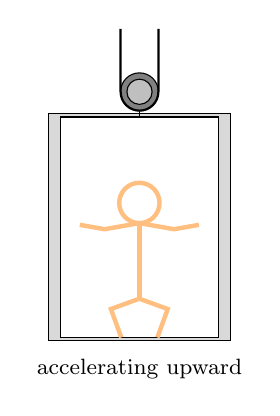
\begin{tikzpicture}[scale=0.8]
        \begin{scope}
          \path (4.2,0) pic{elevator} coordinate (start);


          \begin{scope}[person]
            \draw (start) 
            ++(1.2,0) coordinate (left foot) --
            ++(110:0.6) --
            ++(20:0.6) coordinate (waist) --
            ++(-20:0.6) --
            ++(250:0.6) coordinate (right foot);


            \draw (waist)
              -- ++(90:1.5) coordinate (neck);
            \draw (neck) 
              ++(90:\headsize) circle (\headsize);
            \draw (neck)
              -- ++(-10:0.7) coordinate (right elbow)
              -- ++(10:0.5) coordinate (right hand);
            \draw (neck)
              -- ++(190:0.7) coordinate (left elbow)
              -- ++(170:0.5) coordinate (left hand);
          \end{scope}

          \draw (start) ++(\elevatorwidth/2,-0.5)
            node {\footnotesize accelerating upward};

        \end{scope}
      \end{tikzpicture}

    \part What is the normal force acting on you? \vs 


    \part Calculate what the net force would be if you are accelerating downward.

    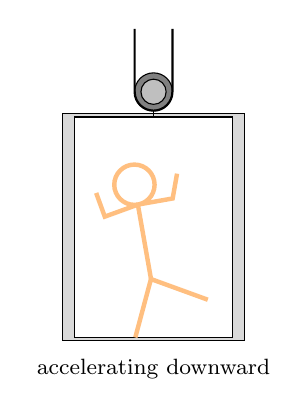
\begin{tikzpicture}[scale=0.8]
      \begin{scope}
        \path (8.4,0) pic{elevator} coordinate (start);

        \begin{scope}[person]
          \draw (start) 
          ++(1.2,0) coordinate (left foot) --
          ++(75:1.2) coordinate (waist) --
          ++(-20:1.2) coordinate (right foot);

          \draw (waist)
            -- ++(100:1.5) coordinate (neck);
          \draw (neck) 
            ++(100:\headsize) circle (\headsize);
          \draw (neck)
            -- ++(10:0.7) coordinate (right elbow)
            -- ++(80:0.5) coordinate (right hand);
          \draw (neck)
            -- ++(-160:0.7) coordinate (left elbow)
            -- ++(110:0.5) coordinate (left hand);
        \end{scope}

        \draw (start) ++(\elevatorwidth/2,-0.5)
          node {\footnotesize accelerating downward};

      \end{scope}
    \end{tikzpicture}
  \end{parts}

\end{questions}

\end{document}